\section{Other tools}
There are a lot of different bibliography management tools out there.
To uncover potential features already in existence we'll try to
uncover what those tools are and what features they provide.

\subsection{Mendeley}
Mendeley is a bibliography management tool developed by Mendeley Ltd.
The focus of the tool is to make it easy to manage and share
references.  Mendeley provides features such as importing PDF-files
and detecting relevant details such as the author, title and DOIs, and
updating entries from online databases using, for instance the DOI.
The target group for Mendeley is students and researchers
\cite{mendeley_features}.

Like BibTeX, Mendeley does not facilitate any systems for detecting
inconsistencies such as spelling errors, revision numbers or initials.
Mendeley can download metainformations based on a DOI which in part
remodies this.  Mendeley does not have any plugin/add on system, so
it's unlikely that there is any third party tools to remedy this. A
search through Mendeley's request database reveals the same as the
testing and features page.  On the request system for Mendelay there
are requests for features such as: spell checking, fixing
capitalization inconsistencies and bulk DOI lookups.
\cite{mendeley_request_spellcheck, mendeley_request_lowercase,
  mendeley_request_capitalization, mendeley_request_bulk_doi}.

\subsection{EndNote and RefMan}
EndNote and RefMan also tools for reference mangement, made by
Thompson Reuters.  RefMan is an older product and Thompson Reuters
recommends using EndNote in stead \cite{refman_switch,
  refman_features}.  There is a lot of focus on the sharing
capabilities and provides tools for PDF import and management, online
lookup of references and Journal abbreviation dection
\cite{endnote_basic_features, endnote_x7_features}.  Their target
group is students and university related groups.

The tools however is only used to format the names when exported or
used as references, mapping from a predefined set of know
abbreviations, the tool does not fix the naming issues internally in
the files\cite{endnote_terms_journals}.  Remedying this by using DOI
lookups also seems to create duplicate entries rather than updating
the current making the issues even worse \remark{Own testing}.
EndNote provides a lot of extra downloads to provide features such as
Bib{\TeX} support, however no downloads were found to remody neither
the lexical nor the consistency concerns \cite{endnote_downloads}.

\remark{Googling reveals a spell checker, find it!}

\subsection{RefWorks}
RefWorks is a web based reference manager targeted at researchers.
RefWorks is developed by ProQuest.  The focus of the tool is to create
an online database for references, so it is available everywhere.

Compared to the other tools the features is very limited and there is
close to no detection of errors.  Two things to note though is that is
contrary to the other tools actually specify how you are supposed to
fill the fields where you fill them and it actually tries to detect if
the author name is malformed, although it only seems to detect if you
type ``John Doe'' rather than ``Doe, John'' as it expects, as can be
seen at figure-\ref{fig:refworks-detect-formatting}.

\begin{figure}[h]
    \centering
    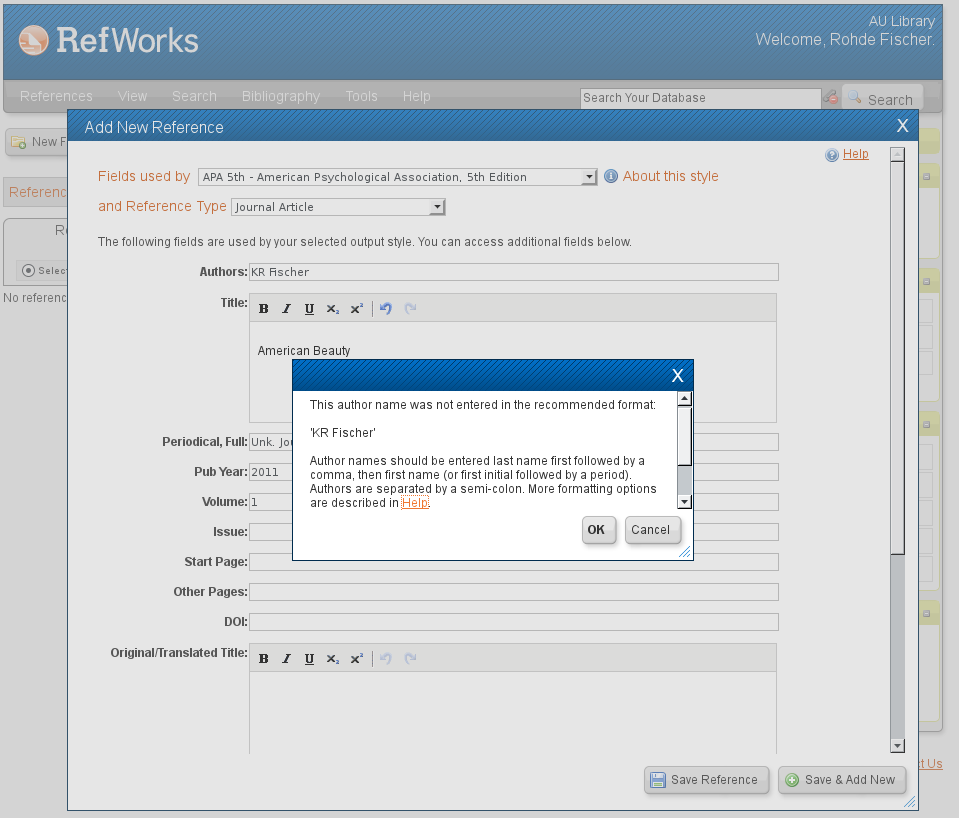
\includegraphics[width=0.8\textwidth]{refworks-detect-formatting}
    \caption{RefWorks detects some formatting on the name field}
    \label{fig:refworks-detect-formatting}
\end{figure}

The fact that RefWorks does not do much more is in part remedied by
most modern browsers, because they tend to include spell checkers for
the input fields.

\subsection{Zotero}
Zotero has a built in spell checker for notes, however the spell
checker is not applied for things like titles, which prevents it from
detecting those errors.  Also it does not seem that it does anything
to detect abbreviations.  Unfortunately Zotero does not have a list of
features directly, apart from some very superficial texts on the front
page \cite{zotero_features}.

Unlike the other systems Zotero has a plugin system, which makes it
possible that a user created plugin for these features exists, however
none was found using the official list of plugins
\cite{zotero_plugins} nor by a normal search engine.

There is a limited mechanism for detecting abbreviations in Zotero, in
its jar-file there is a list of known abbreviations which it can use
to chose the correct abbreviation when exporting, entering a known
abbreviation does not seem to correct it to the non-abbreviated
version.  This list can be manually edited, and overruled
\cite{zotero_abbreviations}

\subsection{Others?}
\remark{Mostly notes to myself}

http://jabref.sourceforge.net/resources.php

%%% Local Variables:
%%% mode: latex
%%% TeX-master: "thesis"
%%% End:
